\subsection{实验目的-了解 MySQL 日志}
了解 MySQL 日志.
%
\subsection{实验原理}
日志是 mysql 数据库的重要组成部分。日志文件中记录着 mysql 数据库运行期间发生的变化,
也就是说用来记录 mysql 数据库的客户端连接状况、SQL 语句的执行情况和错误信息等。当
数据库遭到意外的损坏时,可以通过日志查看文件出错的原因,并且可以通过日志文件进
行数据恢复。
%
\subsection{实验环境}
CentOS6.5:192.168.1.3 MySQL
%
\subsection{实验步骤}
\subsubsection{MySQL 日志介绍}
MySQL 有以下几种日志:
\begin{itemize}
  \item 错误日志:log-err
  \item 查询日志:log
  \item 慢查询日志:log-slow-queries
  \item 二进制日志:log-bin
  \item 更新日志:log-update
\end{itemize}
%
错误日志:记录 MySQL Server 启动和关闭的详细信息、以及运行过程中较为严重的警告和
错误信息,修改错误日志的地址可以在\texttt{/etc/my.cnf} 中添加
\begin{minted}[bgcolor=bg,breaklines=true]{sh}
-log-error = [filename]
\end{minted}
来设置 mysql 错误日志,在 mysql 中是默认开启错误日志的。
\begin{figure}[H]
  \begin{center}
    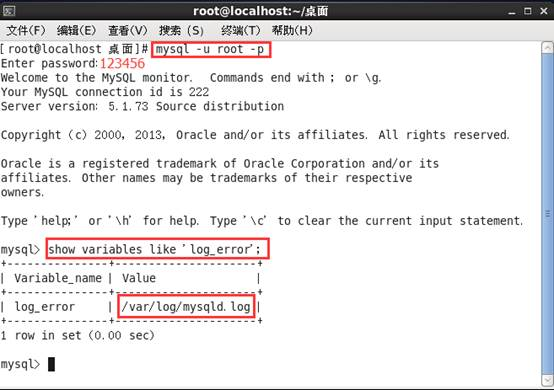
\includegraphics[width=0.40\textwidth]{2_11_1.jpeg}
  \end{center}
\end{figure}
\begin{figure}[H]
  \begin{center}
    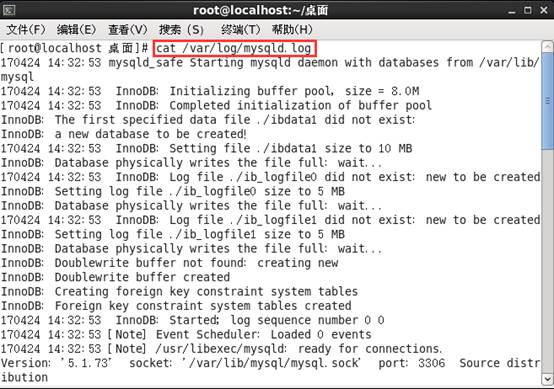
\includegraphics[width=0.40\textwidth]{2_11_2.jpeg}
  \end{center}
\end{figure}

查询日志:记录 mysql 的日常日志,包括查询、修改、更新等的每条 SQL 语句信息。
使用
\begin{minted}[bgcolor=bg,breaklines=true]{sh}
show global variables like '%genera%';
\end{minted}
查看 mysql 是否启用了查询日志。可以看到此时的查询日志是关闭的。
\begin{figure}[H]
  \begin{center}
    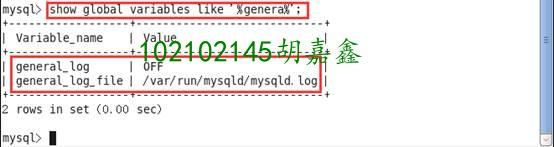
\includegraphics[width=0.40\textwidth]{2_11_3.jpeg}
  \end{center}
\end{figure}

mysql 打开 general log 日志后,所有的查询语句都可以在 general log 文件中输出,
如果打开,文件会非常大,建议调试的时候打开,平时关闭。
查询日志的输出文件可以在
\texttt{/etc/my.cnf} 中添加
\begin{minted}[bgcolor=bg,breaklines=true]{sh}
general-log-file = [filename]
\end{minted}
来开启,也可以使用命令
\begin{minted}[bgcolor=bg,breaklines=true]{sh}
set global general_log = on;
set global general_log = off;
\end{minted}
在 mysql 中打开和关闭。
\begin{figure}[H]
  \begin{center}
    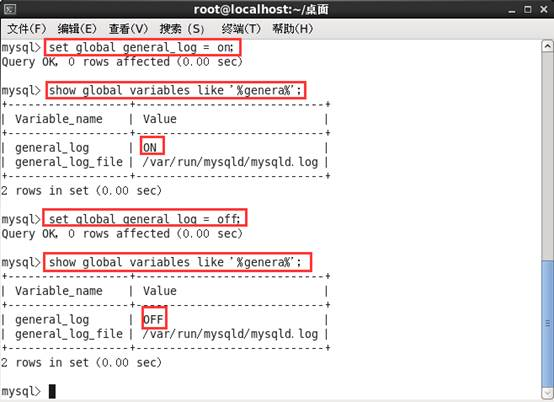
\includegraphics[width=0.40\textwidth]{2_11_4.jpeg}
  \end{center}
\end{figure}

开启查询日志并新建一个名为 simpleware 的数据库。再关闭查询日志,可以看到在查询日
志中记录了创建数据库 simpleware 和关闭查询日志的 SQL 语句。
\begin{figure}[H]
  \begin{center}
    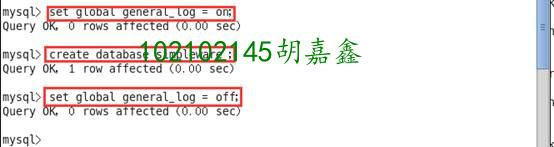
\includegraphics[width=0.40\textwidth]{2_11_5.jpeg}
  \end{center}
\end{figure}
\begin{figure}[H]
  \begin{center}
    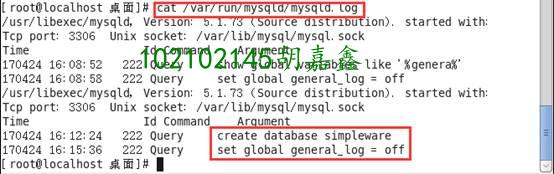
\includegraphics[width=0.40\textwidth]{2_11_6.jpeg}
  \end{center}
\end{figure}

慢查询日志:慢查询日志中记录的是执行时间较长的 query,
可以设一个阀值、将运行时间超过该值的所有 SQL 语句都记录到慢查询日志文件中。
该阀值可以通过参数 \texttt{long\_query\_time} 来设置,默认是 10 秒。
注意:对于运行时间正好等于 \texttt{long\_query\_time} 的情况并不会
被记录,因为在源代码里是判断大于 \texttt{long\_query\_time},而非大于等于。

可以输入命令
\begin{minted}[bgcolor=bg,breaklines=true]{sh}
show variables like '%slow%';
\end{minted}
查看慢查询日志功能是否开启,可以看到此时慢查询日志功能并未开启。
\begin{figure}[H]
  \begin{center}
    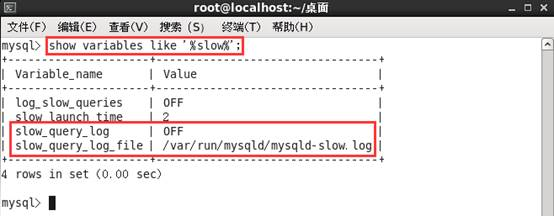
\includegraphics[width=0.40\textwidth]{2_11_7.jpeg}
  \end{center}
\end{figure}

可使用命令
\begin{minted}[bgcolor=bg,breaklines=true]{sh}
set global slow_query_log = on;
set global slow_query_log = off;
\end{minted}
开启或关闭慢查询日志功能。
\begin{figure}[H]
  \begin{center}
    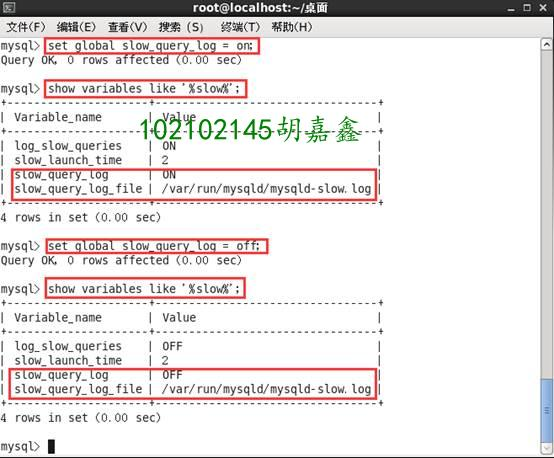
\includegraphics[width=0.40\textwidth]{2_11_8.jpeg}
  \end{center}
\end{figure}

二进制日志文件:记录与修改有关的信息,影响数据潜在的内容的信息,
二进制日志也叫复制日志,默认在数据目录下,
专门查看 mysql 二进制日志文件的命令是 \texttt{mysqlbinlog}。

MySQL 记录二进制日志的格式有三种:
\begin{enumerate}
  \item 基于语句:statement,每一条会修改数据的 sql 都会记录到 master 的 binlog 中,
    slave 在复制的时候,sql 进程会解析成和原来 master 端相同的
    sql 再执行。
  \item 基于行的:row,日志中会记录成每一行数据被修改的形式,
    然后在 slave 端再对相同的数据
    进行修改,只记录要修改的数据,只有 value,
    不会有 sql 多表关联的情况。
  \item 混合模式:mixed,由 MySQL 自己判断以什么方式记录日志,
    MySQL 会根据执行的每一条具体
    的 SQL 语句来区分对待记录的日志形式,
    也就是在 statement 和 row 之间选择一种。
\end{enumerate}

使用命令
\begin{minted}[bgcolor=bg,breaklines=true]{sh}
show variables like '%log_bin%';
\end{minted}
查看mysql 二进制日志文件的配置情况,
log\_bin 用于设定是否启用二进制日志功能,
可以看到此时二进制日志功能未开启。
\begin{figure}[H]
  \begin{center}
    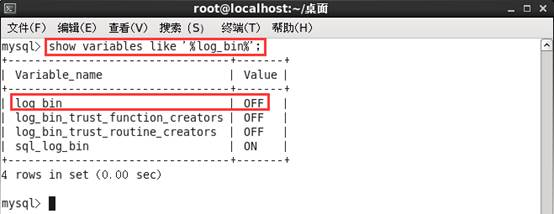
\includegraphics[width=0.40\textwidth]{2_11_9.jpeg}
  \end{center}
\end{figure}
